% notities voor Harman
% we hebben veel overlap, deze dingen kunnen er nog bij
%   - Tom Miller bij SOCIO TECHNICAL
%   - GOVERNANCE zeggen dat Israel zeker geen VSD heeft gebruikt


% notities
% eerst de papers lezen, en daaruit citaties halen


The CHOF structures oversight across three layers: governance, socio-technical layer, and technical. Each of these layers is further analysed across three temporal phases: before, during, and after deployment of the autonomous weapon system. The governance layer concerns the legal and ethical conditions, investigating whether societal values and ethical principles are respected. The socio-technical layer focuses on the stakeholders involved, both the ones operating the system and those personally affected by it. The technical layer looks at the system itself, addressing issues such as automation bias and the system working as a black box, meaning the inner workings of the system are not transparent to users or stakeholders.

\begin{figure}[h]
	\centering
	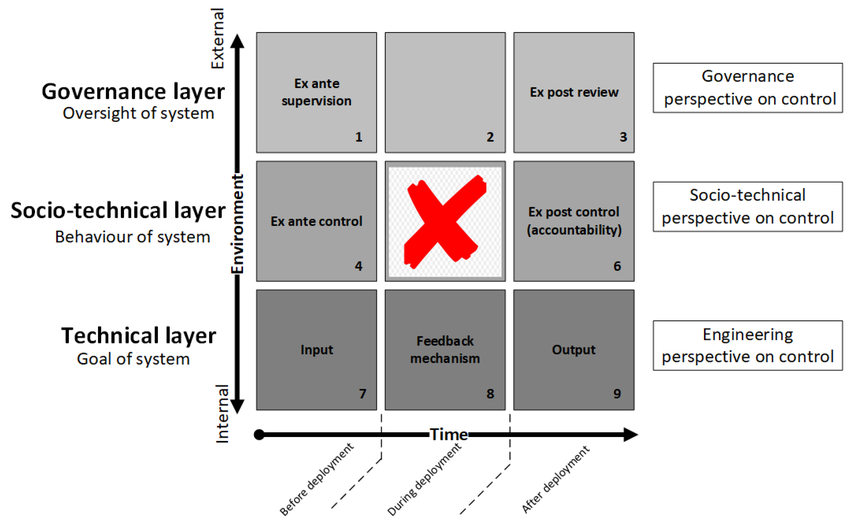
\includegraphics[width=0.8\textwidth]{images/CHOF.png}
	\caption{The CHOF framework for structuring ethical analysis across governance, socio-technical, and technical layers.}
	\label{fig:chof}
\end{figure}


Underpinning all three layers is the Glass Box approach described by~\citet{ijcai2019p802}. This approach translates abstract values, such as human dignity, into observable norms and requirements to be implemented in the the AI system. The Glass Box approach demands that the system's design and operation be transparent and verifiable, allowing for accountability and ensuring that ethical principles are upheld in practice. This is particularly relevant in the context of the IDF's use of the Lavender system, where the opacity of the AI's target recommendations raises significant ethical concerns regarding accountability and meaningful human control.

\begin{figure}[ht]
	\centering
	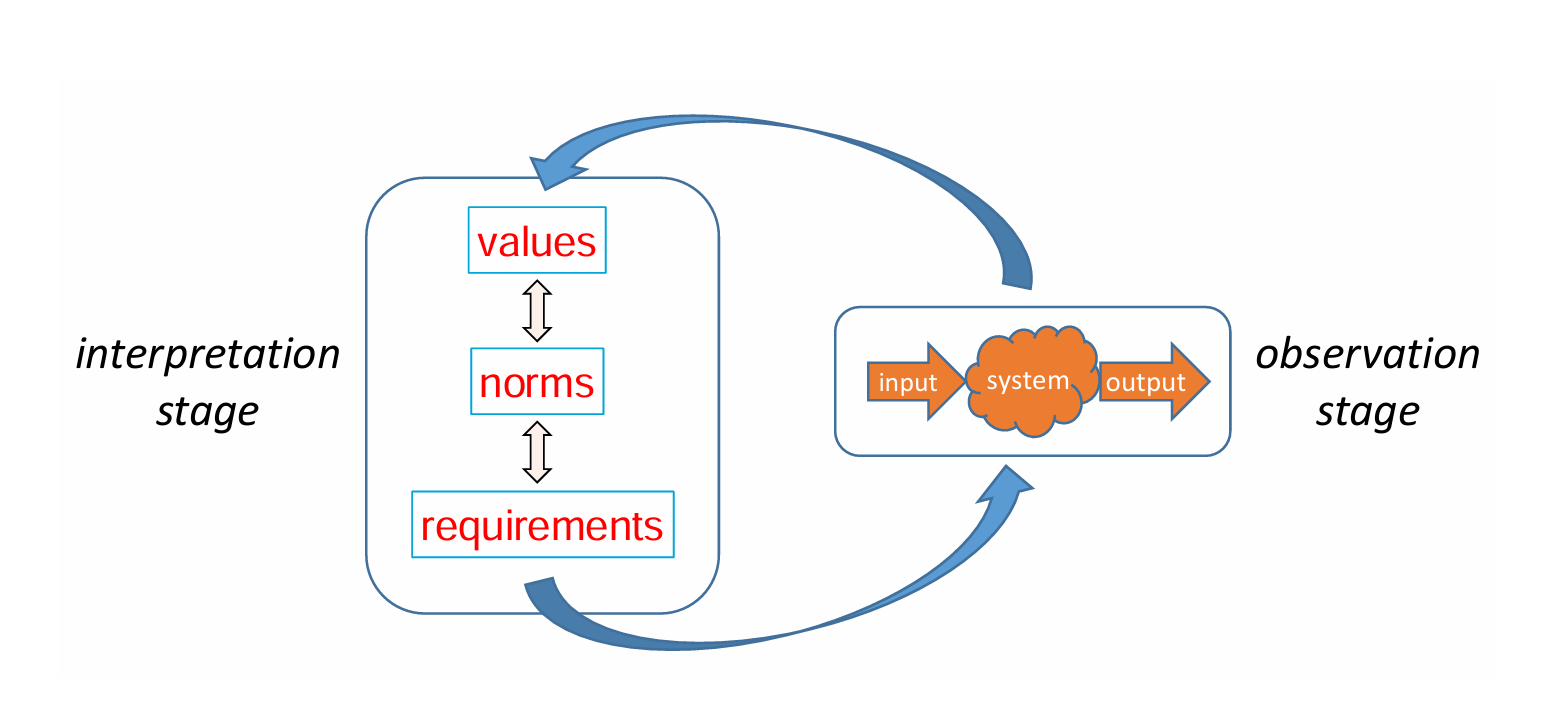
\includegraphics[width=0.8\textwidth]{images/GlassBox.png}
	\caption{The two stages of the Glass-Box Approach: an Interpretation stage, where values are translated into design requirements, and an Observation stage, where we can observe and qualify the behaviour of the system} % de caption komt verbatim uit de oorspronkelijke paper
	\label{fig:glassbox}
\end{figure}


\subsection{Governance Layer}

Article 36 of `Protocol I to the Geneva Conventions' requires countries to conduct legal reviews of new weapons~\citet{icrc_api_article36_1977}. Specifically to determine whether its employment would, in some or all circumstances, be prohibited by international law. These legal reviews examine whether the system can distinguish civilians from combatants, whether it can be used in a way that limits unnecessary suffering, and whether meaningful human control is retained. This article, and the rest of Protocol I, apply to countries that have ratified (formally accepted) it. Israel is one of the few countries that have not~\citep{icrc_api_stateparties} ratified Protocol I. This means that they are not legally obligated to conduct Article 36 reviews of new weapons systems. This forms a gap in governance because there is no legal requirement for Israel to assess the compliance of Habsora with international humanitarian law (IHL) before deployment.


Under International Humanitarian Law (IHL), human commanders remain legally responsible for how weapons are used, even if the system has autonomous functions~\citep{icrc_api_article86_1977}. In reality, commanders are judged on what they knew, or had reason to know, at the time of the decision, not on the basis of hindsight~\citep{henckaerts2005customary}. This creates accountability gaps when an AI system's recommendation leads to civilian casualties. Additionally, in a high-tempo conflict environment, where decisions must be made rapidly, the real-time use of the system can not be effectively monitored, further complicating accountability.

Post-deployment, there is often an absence of meaningful review processes to assess the system's compliance with IHL. It is difficult to attribute responsibility for any violations that may occur, as it may not be clear whether a particular recommendation was generated by the AI or if a human operator overrode it. This lack of transparency hinders accountability and undermines trust in the use of such systems in armed conflict.



\subsection{Socio-technical Layer}

It can be reasonably inferred that the affected stakeholders, Palestinian civilians, were likely not involved in the original design of Habsora. Their values were not elicited to ground the system's targeting logic. The values and needs of those most impacted by the system were not adequately considered.

IDF commanders operating under time pressure may be susceptible to automation bias, where they over-rely on the system's recommendations without sufficient critical evaluation~\citep{parasuraman2010complacency}. This can lead to an erosion of genuine human control, as defined by~\citet{mhcof}. The system's speed and opacity may make it difficult for operators to meaningfully review recommendations, further undermining human control over lethal decisions.

Palestinian civilians are non-consenting stakeholders who bear the consequences of the system's use without any recourse. There is a significant asymmetry between those operating the system and those affected by it, raising ethical concerns about justice and fairness in the deployment of such technologies in armed conflict.

\subsection{Technical Layer}

There were no verifiable, observable requirements anchoring the system's recommendations, and the underlying model was opaque to its operators~\citep{abraham_2024}. This lack of transparency means that operators had no principled basis on which to contest or override a recommendation, as they could not inspect the criteria by which targets were selected.

The speed of output generation is incompatible with meaningful human review. Sources cited by +972 Magazine and Local Call report that human overseers devoted approximately 20 seconds to each target, limiting their verification to whether the target was male, before approving a strike~\citep{abraham_2024}. This effectively reduces the operator to a rubber stamp~\citep{kozlovski2024algorithms}, delegating life-and-death decisions to the system itself. When operators are structurally unable to critically evaluate recommendations due to high throughput constraints, the claim of human oversight becomes procedurally hollow.

The absence of audit trails makes post-hoc verification of norm compliance impossible. Without records of which recommendations were generated, which were overridden, and on what basis, it is impossible to reconstruct the decision-making process after the fact. This forecloses any meaningful accountability mechanism.
% deze citaten kunnen gebruikt worden 
% Sources interviewed by +972 Magazine and Local Call claim that \textquote{during the first weeks of the war, the army almost completely relied on Lavender, which clocked as many as 37,000 Palestinians as suspected militants \textemdash{} and their homes \textemdash{} for possible air strikes.}~\citep{abraham_2024}. A problem that arises in this scenario is that active military personnel start working on a "rubber stamp" basis, where they are not verifying the target lists generated by the AI system and are instead completely relying on the AI system to make decisions that have life and death consequences. One source admitted that human overseers only devoted 20 seconds to each target, were merely checking if the target was male, before approving a strike. This effectively delegates life-and-death decisions to an AI system, which makes establishing accountability and responsibility rather difficult.